%% This is based on bare_conf.tex
%% V1.3
%% 2007/01/11
%% by Michael Shell
%% See:
%% http://www.michaelshell.org/
%% for current contact information.
%%
%% This is a skeleton file demonstrating the use of IEEEtran.cls
%% (requires IEEEtran.cls version 1.7 or later) with an IEEE conference paper.
%%
%% Support sites:
%% http://www.michaelshell.org/tex/ieeetran/
%% http://www.ctan.org/tex-archive/macros/latex/contrib/IEEEtran/
%% and
%% http://www.ieee.org/
%\documentclass[conference,a4paper]
\documentclass[a4paper,10pt]{article}
\usepackage{cite}
\usepackage[pdftex]{graphicx}
\usepackage[cmex10]{amsmath}
\usepackage{fixltx2e}
\usepackage{url}

\begin{document}
%
% paper title
% can use linebreaks \\ within to get better formatting as desired
\title{ESG Seminar Experiment \\ Dynamic Dataflow and Open Event Machine}

% author names and affiliations
% use a multiple column layout for up to three different
% affiliations
\author{Risto Vuorio}
%\IEEEauthorblockA{Your Association}

% make the title area
\maketitle

\begin{abstract}
\end{abstract}

\section{Introduction}
Dataflow models of computation are well suited for stream processing tasks. There are many kinds of dataflow models but in this experiment the focus is on dynamic dataflow. Dynamic dataflow models have good powers of expression. The dynamic dataflow graphs allow for conditional execution of actors, which can be used for the construction of iterations and many other logic flows in the dataflow graphs. In general the resulting graphs are not statically schedulable. The dynamic scheduling of the actors is left for the dataflow framework.~\cite{semmapaperi} In this experiment a program of which high level structure is compatible with dynamic dataflow is implemented using Open Event Machine.

\section{Experiment Construction}
Open Event Machine is a runtime system for concurrent programming developed by Nokia Solutions and Networks. A good introduction to OpenEM can be found in~\cite{dippa}. In this experiment dynamic dataflow actors are mapped to OpenEM execution objects. The OpenEM framework does not support explicit representations of the execution graph. The dynamic dataflow model corresponding to the measured program is presented in figure~\ref{fig:ddf_model}. 

\begin{figure}[!h]
    \centering
        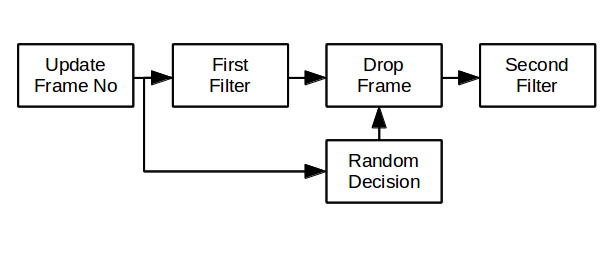
\includegraphics[width=30pc]{ddf_model.png}
        \caption{Dynamic Dataflow model corresponding to the experiment program}
        \label{fig:ddf_model}
\end{figure}

\bibliographystyle{IEEEtran}
\bibliography{papers}

\end{document}

